\section{灌溉需求与分水配额的失配}

\begin{figure}[!ht]
    \centering
    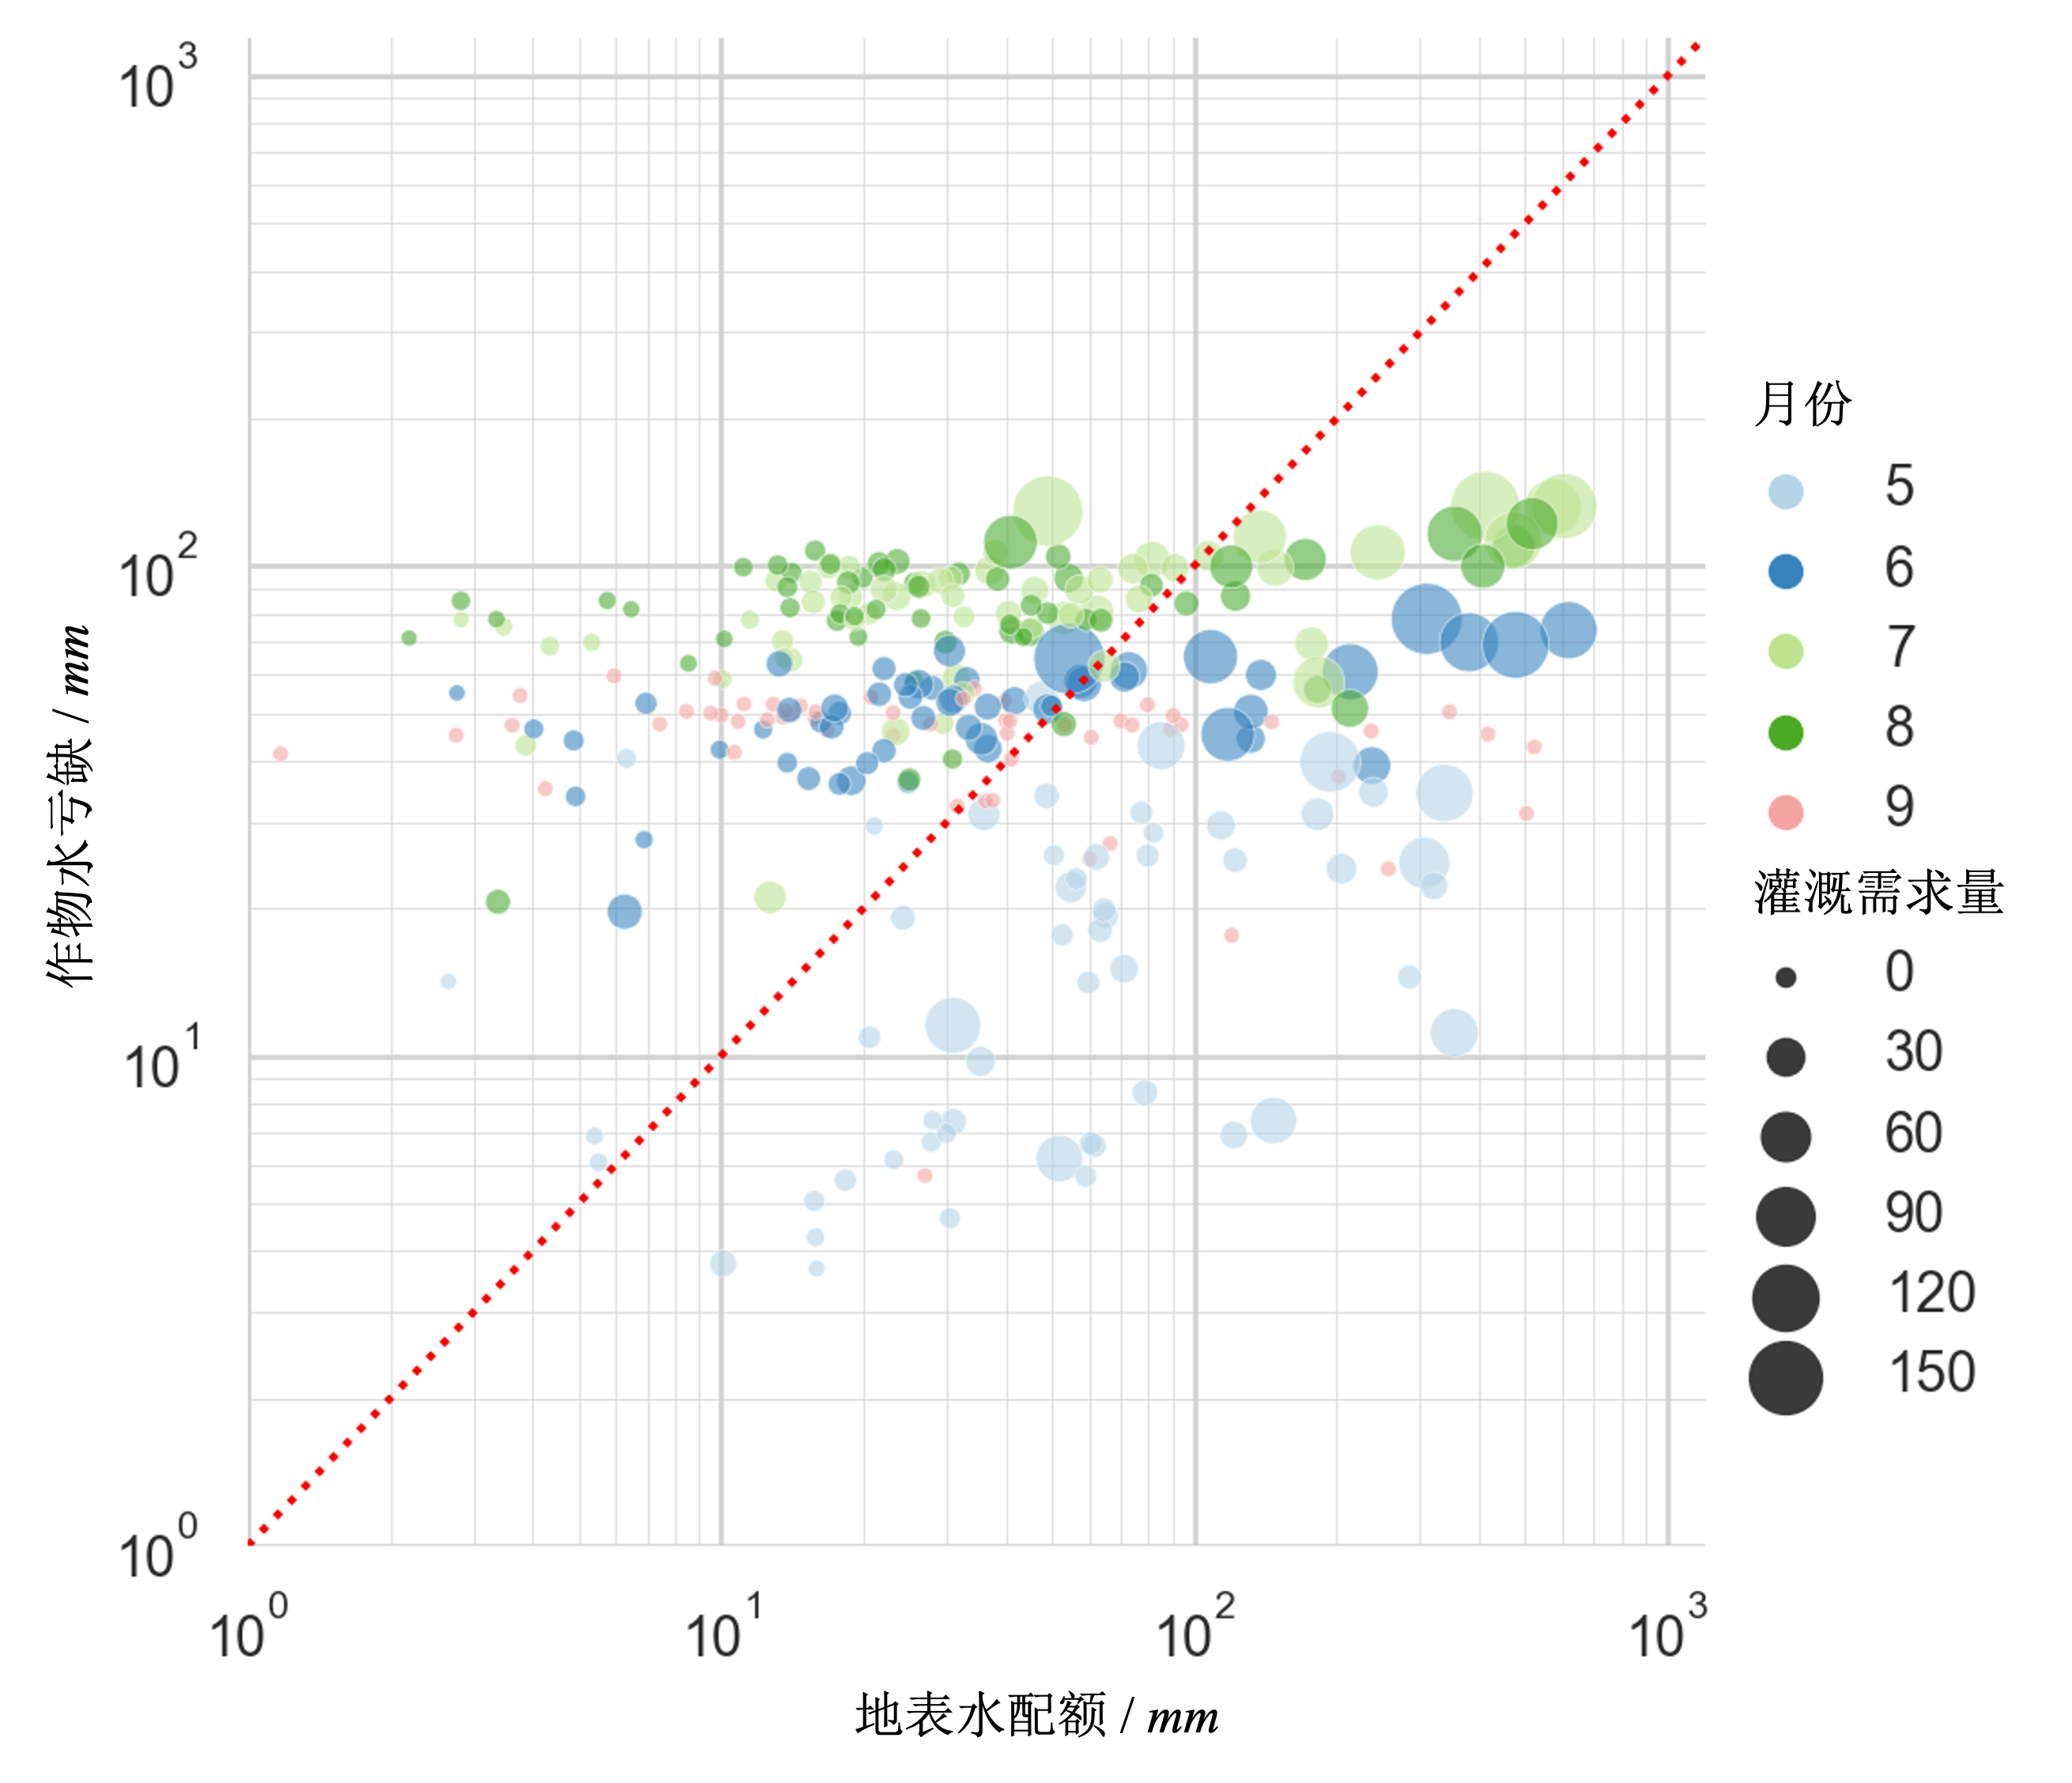
\includegraphics[width=0.8\textwidth]{img/ch6/ch6_matches.png}
    \caption{黄河流域各地级市主要粮食作物生长季水亏缺与地表水配额}\label{ch6:fig:matches}
\end{figure}

图\ref{ch6:fig:matches}展示了月尺度水资源配额与作物水资源亏缺的关系。
红色虚线表示两者的$1:1$线,右侧表示配额大于作物需求,左侧则表示配额小于作物的绝对用水需求。
可见黄河地表水配额与作物水亏缺存在时空分布不匹配现象,因为如果两者匹配得很好,大多数气泡点应该落在$1:1$线上。
气泡的大小代表了统计数据中的地区实际总灌溉用水量,可见水需求量较大的大型灌区也获得了较多的用水配额,容易出现配额供给大于实际作物需求的情况,而在规模偏小的地区则存在水配额供小于求的情况。
此外,气泡的颜色代表了作物生长季的不同月份,可见$6$月到$9$月之间的水资源供需失配情况分布比较相似,都是高需水地区有富余,低需水地区存在不足;仅在作物生长的初期($5$月)的配额普遍出现水资源配额富余的情况。

\begin{figure}[!ht]
    \centering
    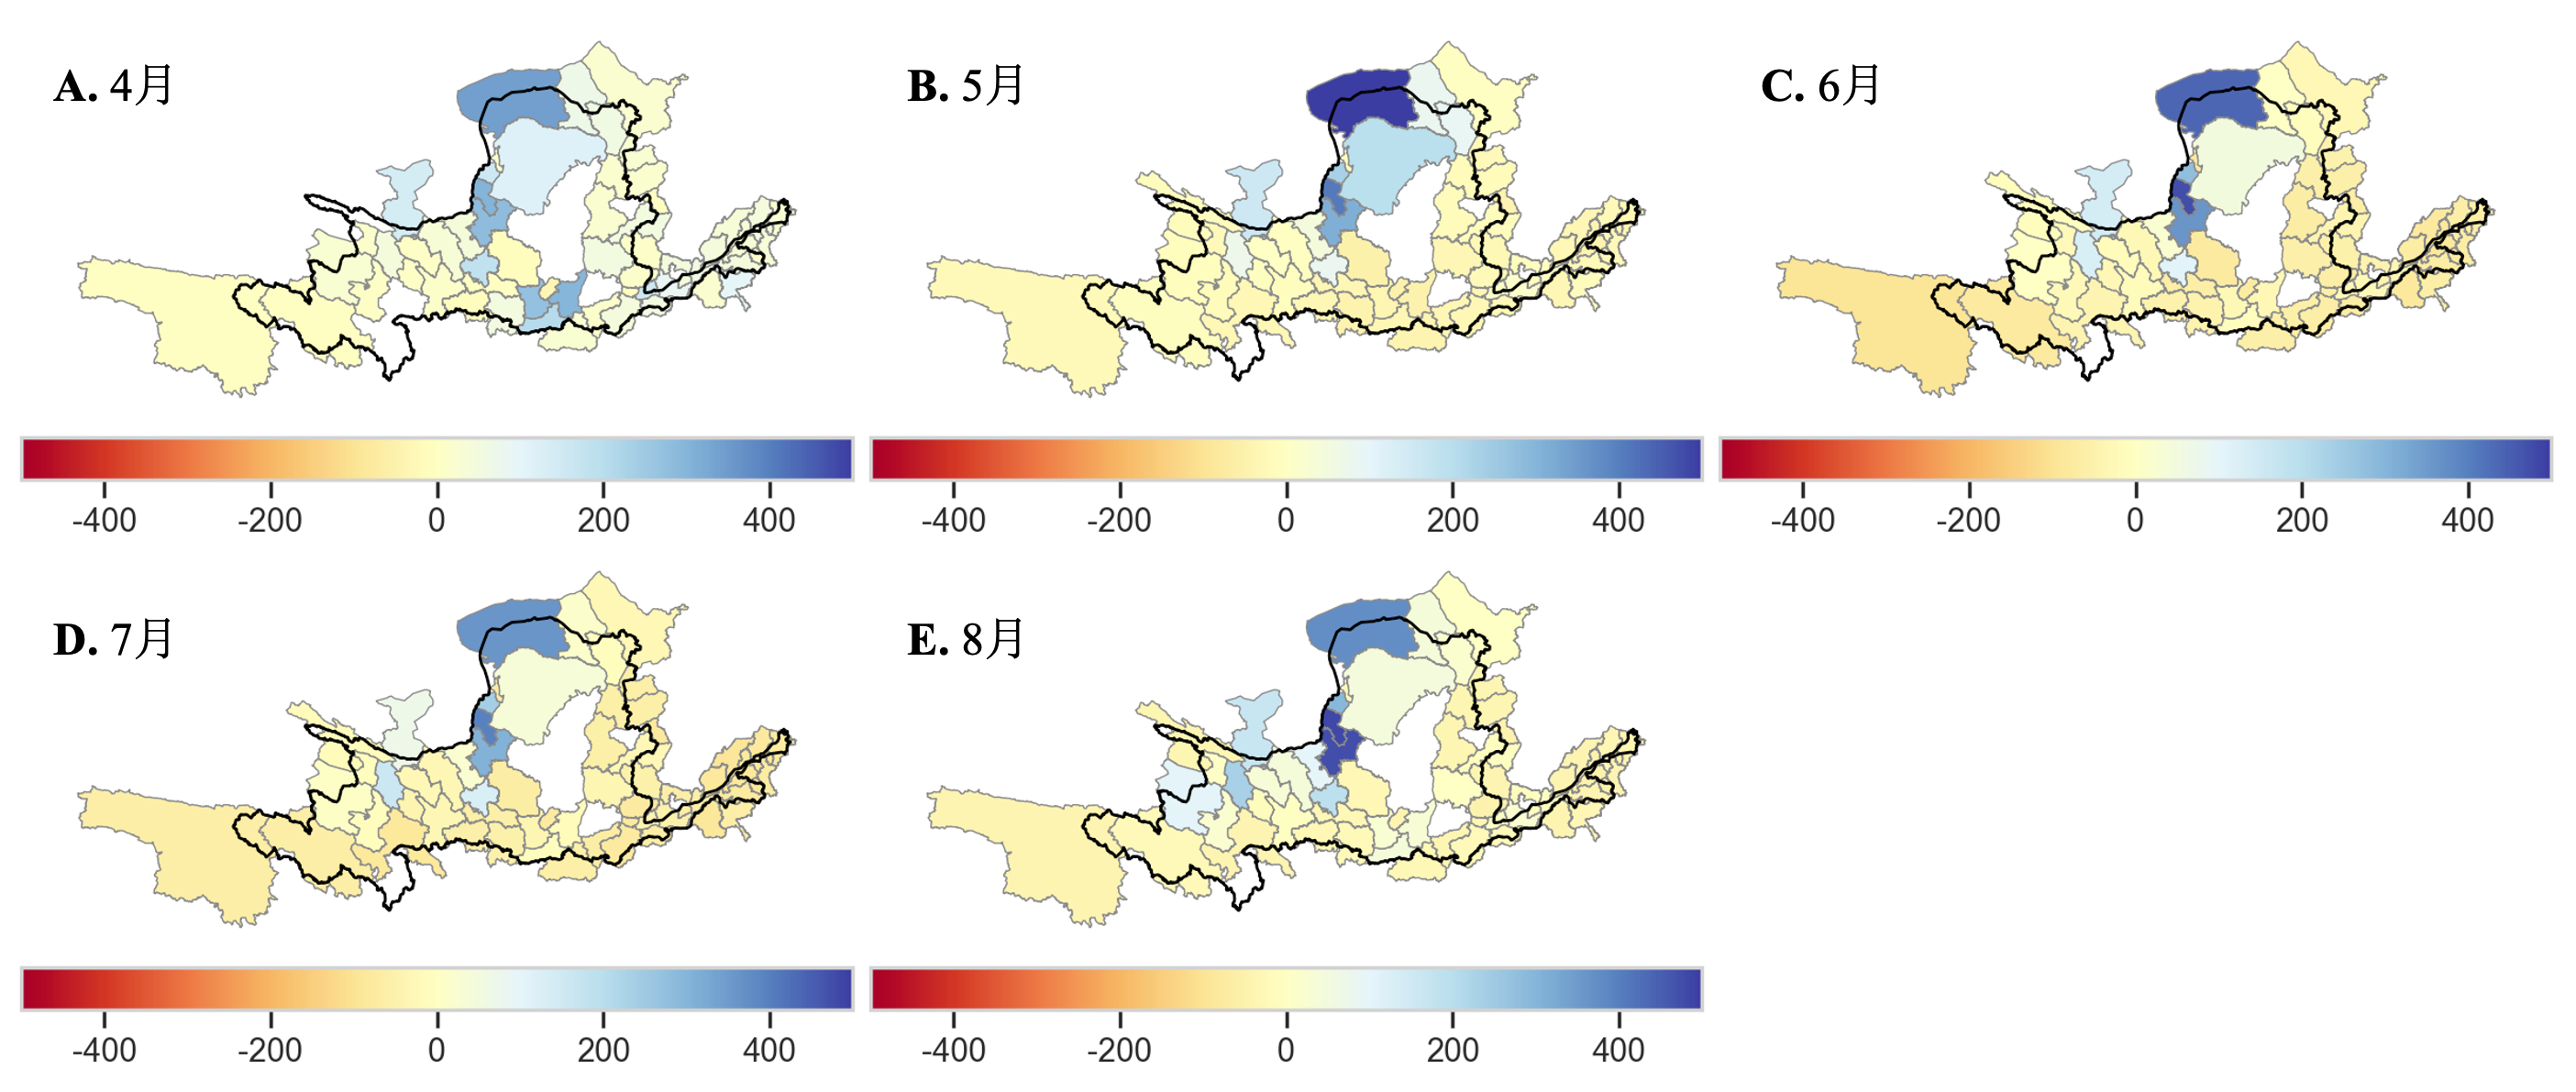
\includegraphics[width=\textwidth]{img/ch6/ch6_deficits_map.png}
    \caption[黄河地表水配额与主要粮食作物需水量之差]{黄河地表水配额与主要粮食作物需水量之差(单位$mm$),$A \textendash{} E$分别表示4月至8月的情况。}\label{ch6:fig:deficits_maps}
\end{figure}

进一步将尺度水资源配额与作物水资源亏缺的差值映射到地图上(图\ref{ch6:fig:deficits_maps}),可以发现大多数地区五月的配额仍属于供需平衡的状态,但河套灌区已经有非常明显的配额富余。
而六、七月的供需失配情况更加严重,不仅河套灌区作物需求和配额供给之间的差异部分地区有超过$500~mm$的配额富余,黄河流域的其它地区则平均有$100~mm$左右的配额亏缺,尤其是下游河南、山东的灌区,均有严重的配额不足情况。

% \section{用水者对分水制度变化的响应}

% 本研究根据每年的灌溉面积确定主体数量,水稻、玉米、小麦各类粮食作物灌溉主体的数量分布如图\ref{ch6:fig:agents}所示,其中小麦种植面积最广,玉米其次,水稻仅部分地区有少量分布,地级市尺度上平均生成的主体数量不足$2$个。
% 将1987年“八七”分水方案出台后的每三年分成一个时间段,将此地表水配额灵活时期分为初期($1988 \textendash{} 1991$)、中期($1992 \textendash{} 1994$)、后期($1995 \textendash{} 1998$)三个时段,诸省份农业主体在不同时期对水资源配额的合作比例如图\ref{ch6:fig:compliacne}所示。
% 可见,由于社会系统存在决策的演化传播,违背分水制度进行超额取水的主体比例会随时间变化,大多数省份的主体的变化趋势都是在初期到中期合作比例显著下降,在中期到末期又上升的“V”形变化趋势。
% 整体来说,大多数省份在1987年“八七”分水制度出台后的六年时间里都偏向于违背此分水配额,从前期到中期选择合作策略的比例都呈现明显的下降趋势(仅宁夏除外)。
% 在种植三种不同粮食作物的主体中,水稻对制度变化更敏感,合作策略的变化幅度也较大;种植玉米的主体在中期至后期合作的比例趋于稳定;种植小麦的农户面对用水配额选择不合作的占比则持续增加。

% \begin{figure}[!ht]
%     \centering
%     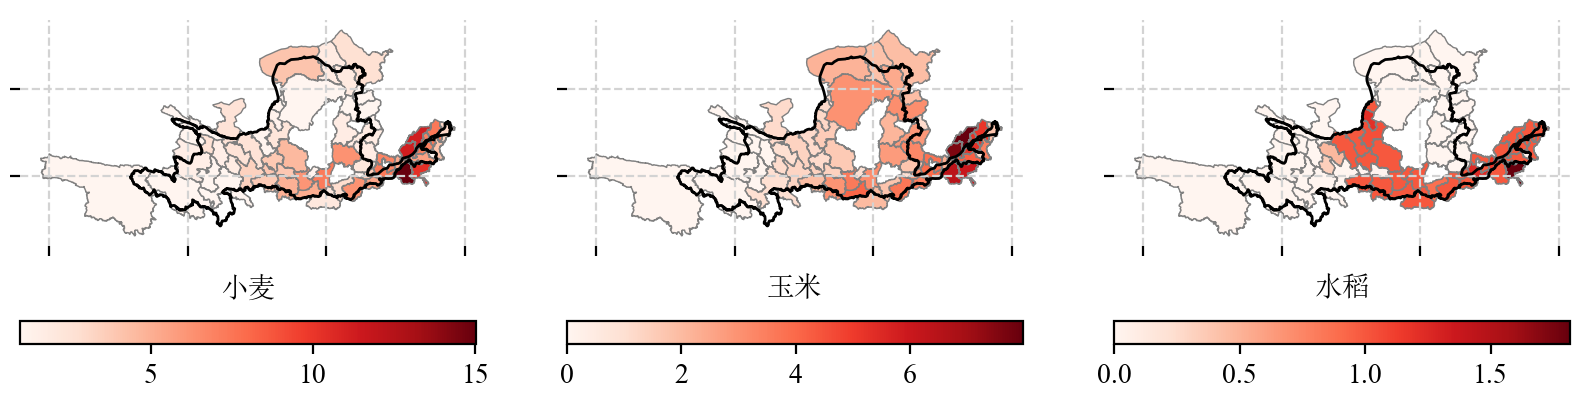
\includegraphics[width=\textwidth]{img/ch6/ch6_agents.png}
%     \caption{黄河流域三种主要粮食作物的平均灌溉主体数量分布}\label{ch6:fig:agents}
% \end{figure}

% \begin{figure}[!ht]
%     \centering
%     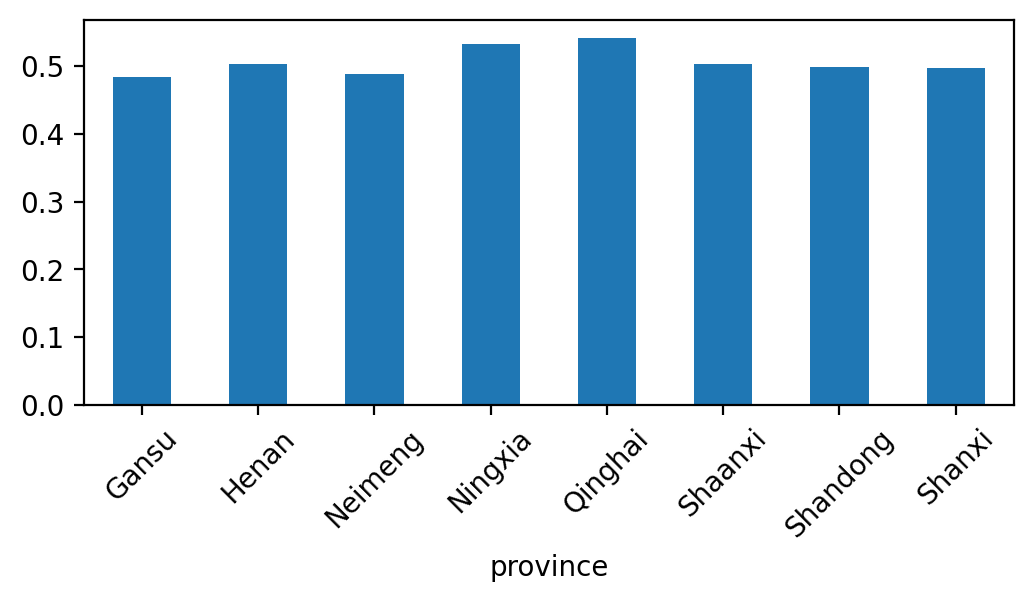
\includegraphics[width=\textwidth]{img/ch6/ch6_compliance.png}
%     \caption{$1988$年至$1997$年主体博弈决策中选择合作的主体比例}\label{ch6:fig:compliacne}
% \end{figure}

\section{灌溉用水来源对分水制度变化的响应}

本研究所建立的模型可以模拟黄河流域主要粮食作物种植中各类水源(降水、地表水、地下水)的使用情况。
天然降水是黄河流域大多数省份粮食作物生长的主要水源,但在河套灌区的宁夏和内蒙古两自治区,地表水灌溉的占比更大(见图\ref{ch6:fig:sources})。
此外,各省总体上都保持了蓝水使用占比持续下降的趋势,但是对用蓝/绿水比例的影响并不明显,仅青海和山西存在一定程度的突变。
另外,通过分析地表水和地下水的使用量的分布情况,发现地表水使用量前$50\%$的主体在1987年到1987年之间用水量进一步扩大,而另外$50\%$用水量较小的地表水使用量则仍分布在约$100~mm$以下,而地下水和灌溉用水的分布在两次分水制度前后的变化不大(图\ref{ch6:fig:sources_change})。


\begin{figure}[!ht]
    \centering
    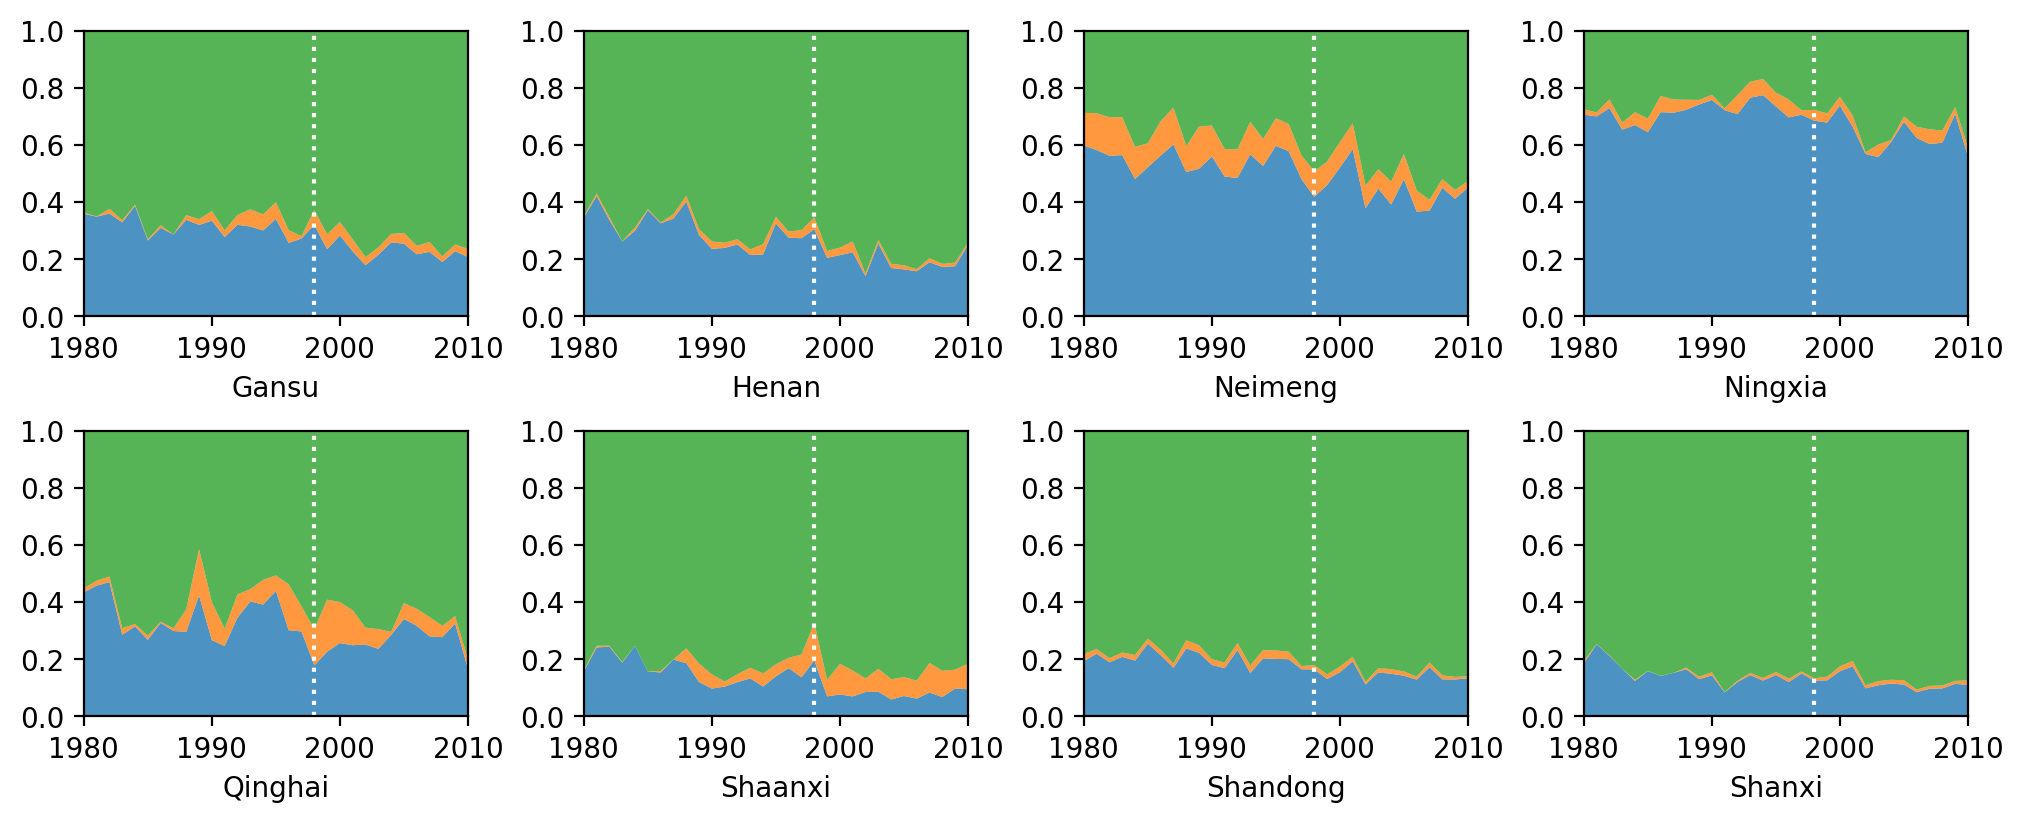
\includegraphics[width=\textwidth]{img/ch6/ch6_green_blue_water.png}
    \caption{黄河流域各省主要粮食作物灌溉用水来源的比例变化}\label{ch6:fig:sources}
\end{figure}

\begin{figure}[!ht]
    \centering
    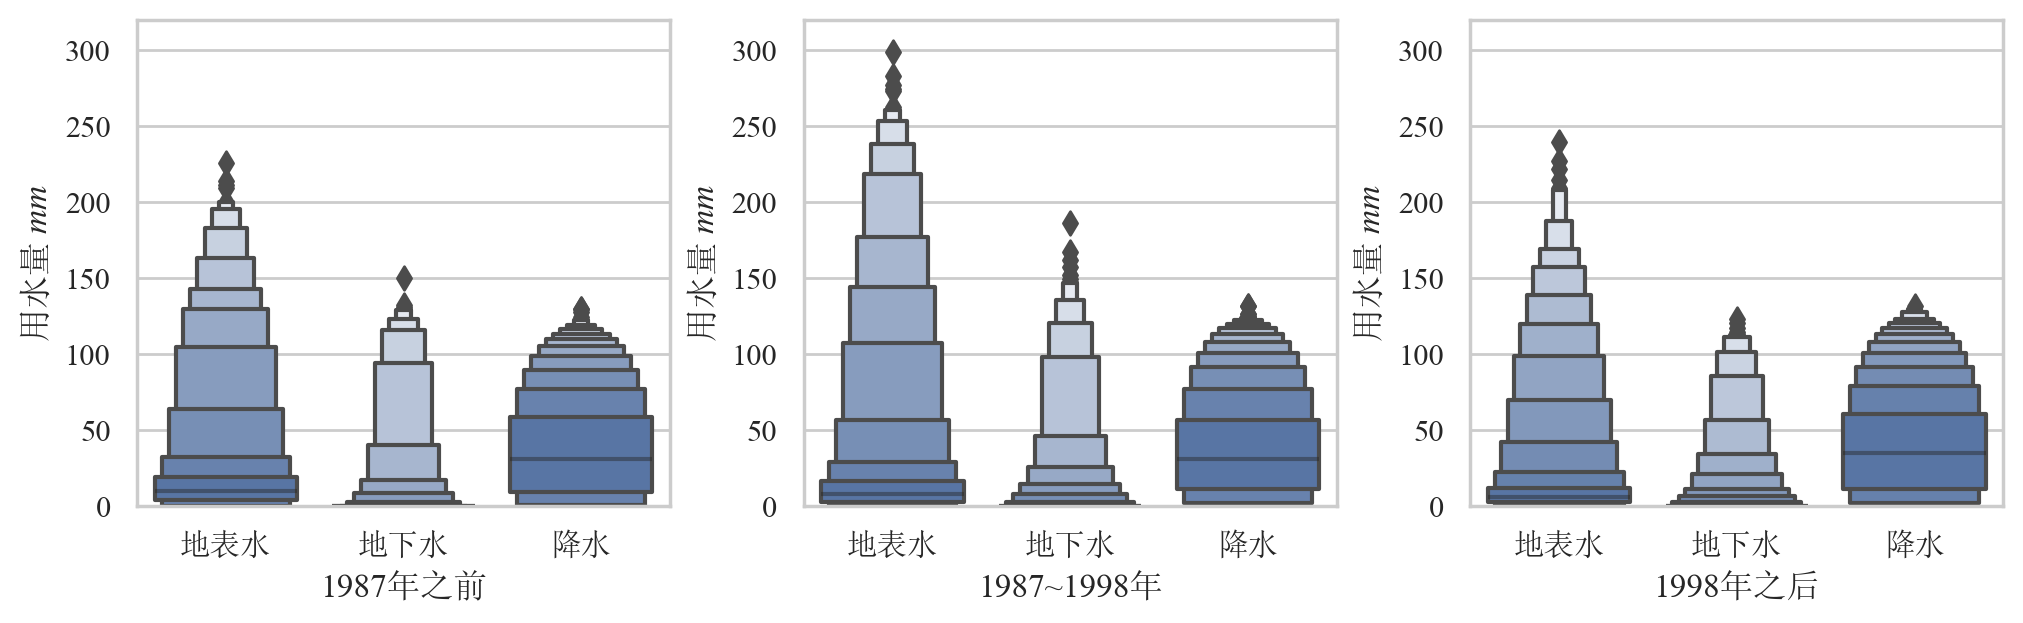
\includegraphics[width=\textwidth]{img/ch6/ch6_sources_change.png}
    \caption{黄河流域分水制度变化前后灌溉用水来源的供水量分布}\label{ch6:fig:sources_change}
\end{figure}

分水制度变化对黄河流域的地下水使用量带来的影响较为明显,且黄河上(头道拐以上)、中(花园口以上)、下游地区对这种变化的响应过程有所差异。
具体来说,下游地区地下水开采量在$1980$年至$2010$年始终维持在较低水平且变化不大;中游地区在此期间则持续增加地下水的开采量;上游在1987年分水制度提出之初期先是增加了地下水开采,在$1991$年左右出现下降趋势(图\ref{ch6:fig:groundwater})。

\begin{figure}[!ht]
    \centering
    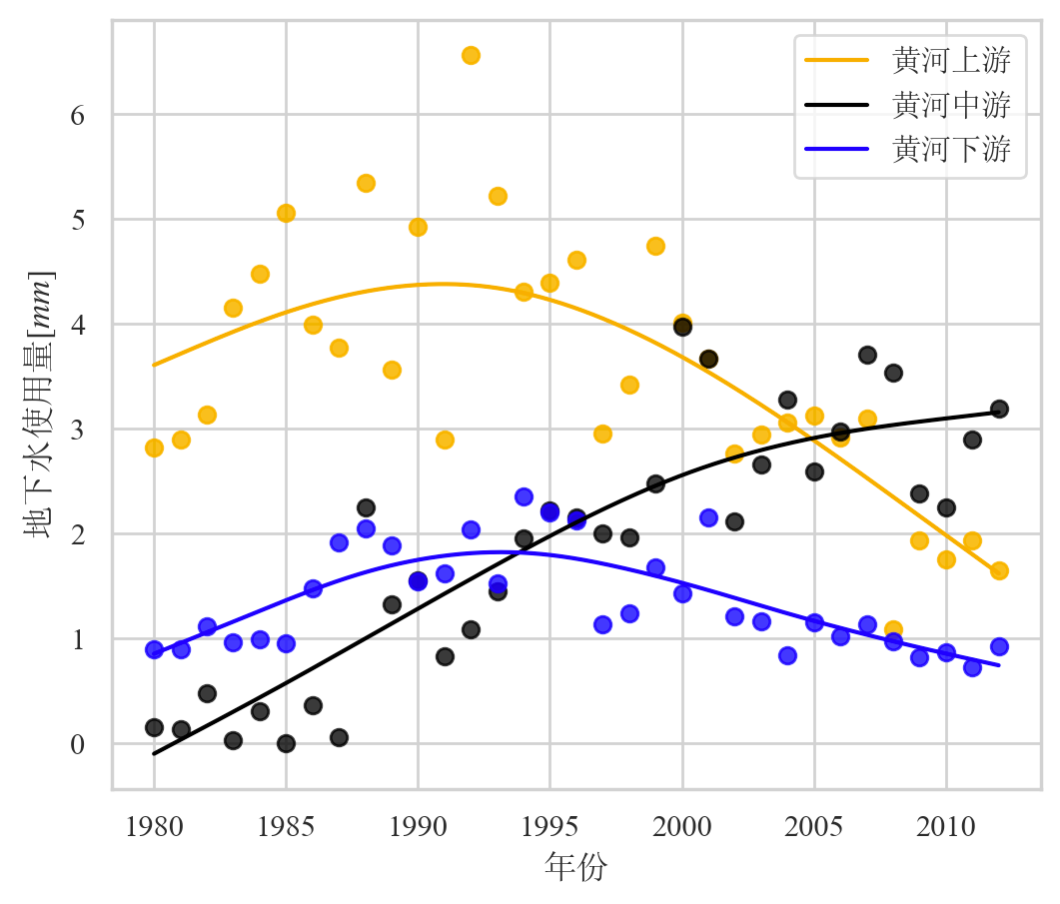
\includegraphics[width=0.6\textwidth]{img/ch6/ch6_groundwater.png}
    \caption{黄河流域不同区域地下水开采量随时间的变化趋势}\label{ch6:fig:groundwater}
\end{figure}